\documentclass{article}
\usepackage[T2A]{fontenc}
\usepackage[utf8]{inputenc}
\usepackage[english,russian]{babel}
\usepackage{amsmath,amssymb}
\usepackage[pdftex]{graphicx}
\usepackage{fancyhdr} 
\usepackage[left=3cm,right=3cm,
top=2.5cm,bottom=2.5cm,bindingoffset=0cm]{geometry}
\begin{document}
\selectlanguage{russian}
\fancyhead[CO]{ТЕОРЕМА МОРЛЕЯ}
\pagestyle{fancy}
ТЕОРЕМА МОРЛЕЯ
\\Э.Г.Готман
\\(г.Арзамас)
\\З.А.Скопец
\\(г.Ярославль)
\\На первой странице обложки нашего журнала помещен чертеж к теореме Морлея. Любителям математики хорошо известна эта удивительная теорема элементарной геометрии о трисектрисах труеугольника . Она была сформулирована американским математиком Ф. Морлеем (1860-1937). Первые доказательства теоремы Морлея опубликованы в 1909 г. Позднее появилось более десятка новых доказательств, но довольно сложных по сравнению с ее простой формулировкой.
\par Предлагаемое ниже элементарное доказательство доступно учащимся старших классов и может быть расмотрено на занятиях математического кружка. 
\par \textbf{Теорема.}  Трисекрисы углов треугольника, примыкающие к одной стороне, попарно пересекаются в точках, являющихся вершинами равностороннего треугольника. 
\par Трисектрисами угла называют прямые, проходящие через вершину угла и делящие его на три равные части. 
\par \textbf{Доказательство.} Пусть трисектрисы углов данного треугольника $ABC$, примыкающие к сторонам $BC$, $CA$ и $AB$, пересекаются в точках $X$, $Y$ и $Z$
\\
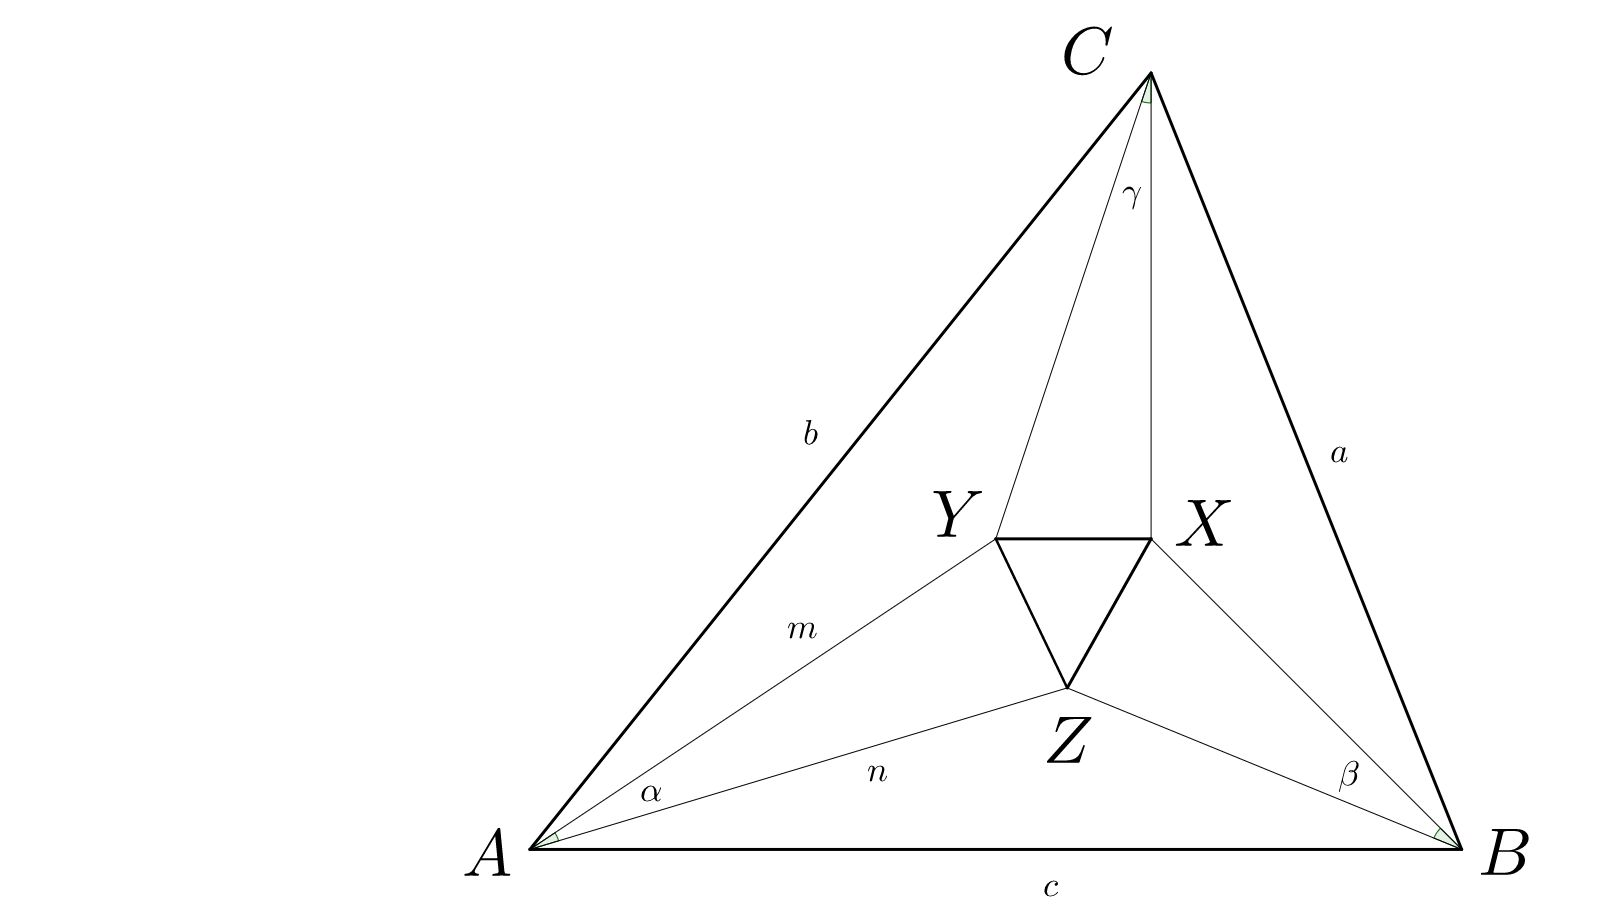
\includegraphics[scale=0.25]{morley1.png}(рис.1)
\\
\par Введем обозначения: $A=3\alpha$, $B=3\beta$, $C=3\gamma$,$ \mid AY \mid=m$, $\mid AZ\mid=n$. Длины сторон треугольника $ABC$ будем обозначать через $a$,$b$ и $c$.
\par Вычислим величины углов $AZY$ и $BZX$. 
\par Так как $3\alpha+3\beta+3\gamma=180^{\circ}$, то $\alpha+\beta+\gamma+60^{\circ}$ и $\alpha+\beta=60^{\circ}-\gamma$. Применив теорему синусов к треугольнику $AZB$, получим $$\frac{n}{c} =\frac{\sin\beta}{\sin(\alpha+\beta)},$$
отсюда $$n=\frac{c\sin\beta}{\sin(\alpha+\beta)}=\frac{c\sin\beta}{\sin(60^{\circ}-\gamma}.$$
Аналогично находим, что $$m=\frac{b\sin\gamma}{\sin(60^{\circ}-\beta)}.$$
Из треугольника $ABC$ по теореме синусов  имеем $$\frac{b}{c}=\frac{\sin3\beta}{\sin 3\gamma}.$$
Следовательно, $$\frac{m}{n}=\frac{\sin3\beta\sin\gamma\sin(60^{\circ}-\gamma)}{\sin 3\gamma\sin\beta\sin(60^{\circ}-\beta)}.$$
Упростим это равенство, применив тождество $\sin 3 \beta=4 \sin \beta \sin(60^{\circ}+\beta)\sin(60^{\circ}-\beta)$. Получим: $$ \frac{m}{n}=\frac{\sin(60^{\circ}+\beta)}{\sin(60^{\circ}+\gamma)}.$$
Теперь уже без всяких вычислений можно доказать, что интересующие нас углы $AZY$ и $AYZ$ треугольника $AYZ$ равны $60^{\circ}+\beta$ и $60^{\circ}+\gamma$.
\par Действительно, так как $\alpha+\beta+\gamma=60^{\circ}$, то существует треугольник с углами $60^{\circ}+\beta$, $60^{\circ}+\gamma$ и $\alpha$, а отношение его сторон, заключающих угол $\alpha$, равно $$\frac{\sin(60^{\circ}+\beta)}{\sin(60^{\circ}+\gamma)}=\frac{m}{n}.$$
Поскольку $\widehat{YAZ}=\alpha$, треугольник $AYZ$ подобен такому треугольнику. Тогда $$\widehat{AZY}=60^{\circ}+\beta \mbox{ и } \widehat{AYZ}=60^{\circ}+\gamma.$$
\par Точно так же докажем, что $\widehat{BZX}=60^{\circ}+\alpha$.  А так как $\widehat{AZB}=120^{\circ}+\gamma$ и $\widehat{YZA}+\widehat{AZB}+\widehat{BZX}=(60^{\circ}+\beta)+(120^{\circ}+\gamma)+(60^{\circ}+\alpha)=300^{\circ}$
, то    $\widehat{XZY}=60^{\circ}.$ 
\par Аналогично докажем, что каждый из двух других углов треугольника $XYZ$ также равен $60^{\circ}$. Значит, треугольник $XYZ$ -- равносторонний.
\par При попытке доказать теорему Морлея геометрически возникают большие трудности. Их удается преодолеть, если действовать в обратном порядке: сначала построить равносторонний треугольник $XYZ$, а затем исходный треугольник $ABC$. Такого рода доказательство имеется в книге Г.С.М. Кокстера  $\ll$Введение в геометрию$\gg$ (М.: Наука, 1966, с. 44-45).
\par Теорему Морлея можно обобщить, если рассматривать кроме внутренних еще и внешние трисектрисы треугольника (прямые, делящие на три равные части внешние углы треугольника, а также углы, дополняющие углы треугольника до $360^{\circ}$).
\par Знаменитый французский математик А. Лебег в 1939 г. опубликовал статью, в которой, используя элементарные средства, доказал, что среди точек пересечения всех трисектрис треугольника можно указать 27 троек, являющихся вершинами равносторонних треугольников. 
\par В частности, трисектрисы внешних углов треугольника $ABC$, примыкающие к одной и той же стороне, попарно пересекаются в точках, являющихся вершинами равностороннего треугольника (рис. 2).
\\
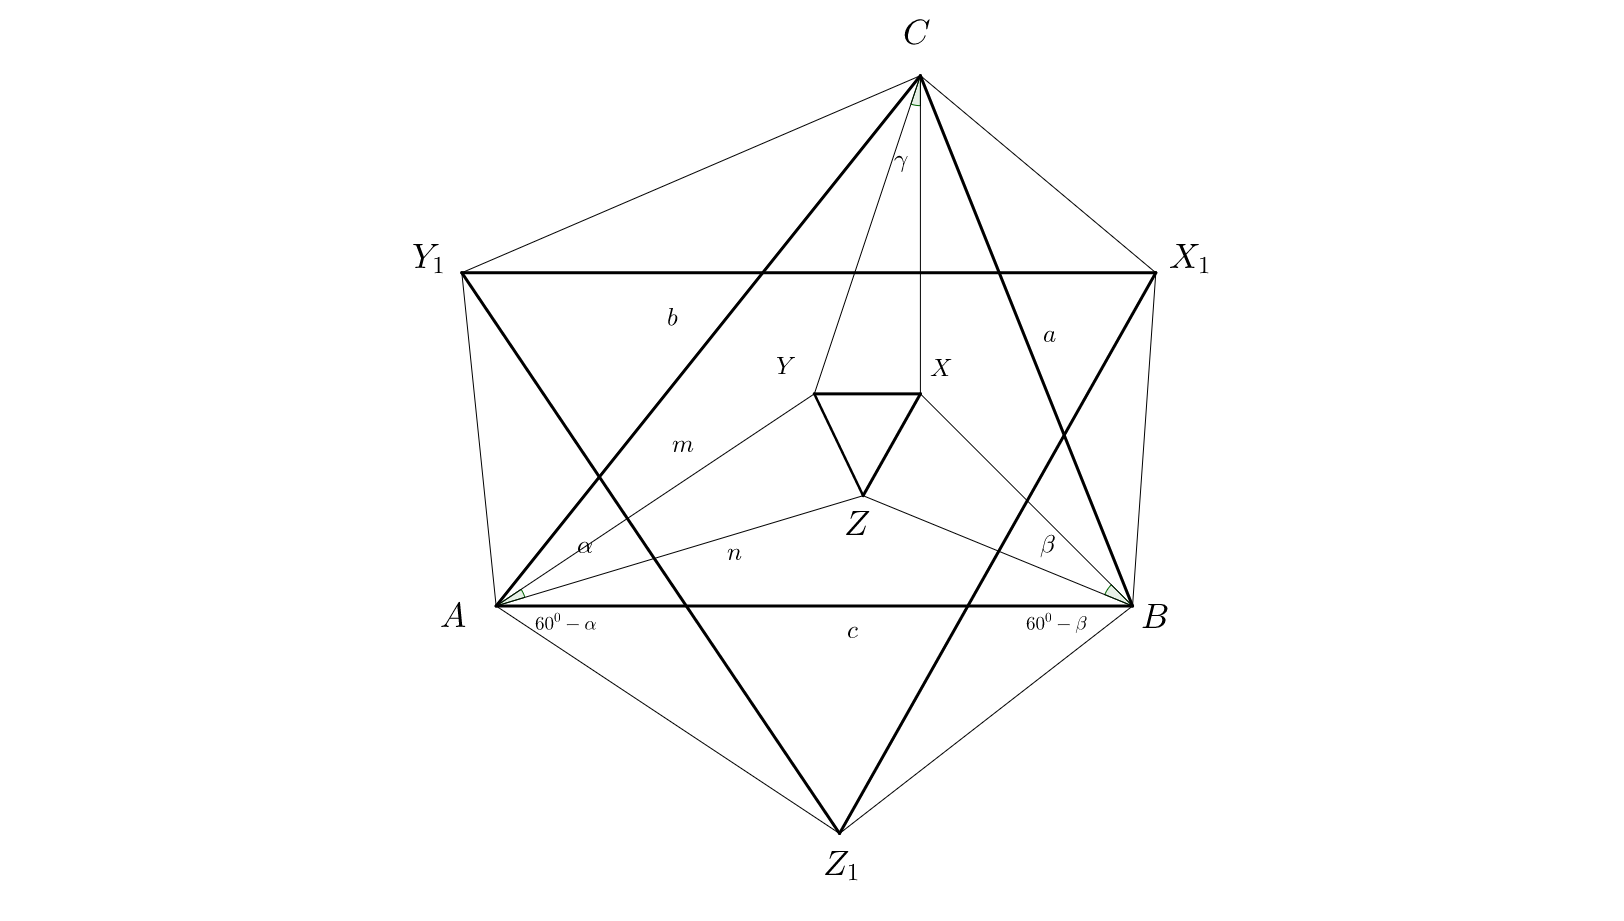
\includegraphics[scale=0.25]{morley2.png}(рис.2)
\par Простое и экономное доказательство можно получить, применив тригонометрию. Если $X_1$,$Y_1$,$Z_1$ -- точки пересечения указанных трисектрис, то, пользуясь теоремой синусов, как в приведенном выше доказательстве, устанавливаем, что углы $Z_1$ и $Y_1$ треугольника $A$ $Y_1$ $Z_1$ равны соответственно $\beta$ и $\gamma$, а каждый из углов треугольника $X_1$ $Y_1$ $Z_1$ равен $60^{\circ}$. Кроме того, легко установить, что стороны треугольника $X_1$$Y_1$$Z_1$ соответственно параллельны сторонам треугольника $XYZ$. 
\par Эффектное доказательство полной обобщенной теоремы Морлея можно провести, используя аппарат комплексных чисел.
\end{document}
